\documentclass{article}

\PassOptionsToPackage{numbers, compress}{natbib}
\usepackage[sglblindworkshop]{neurips_2026}
\usepackage[utf8]{inputenc}
\usepackage[T1]{fontenc}
\usepackage{hyperref}
\usepackage{url}
\usepackage{booktabs}
\usepackage{amsfonts}
\usepackage{amsmath}
\usepackage{nicefrac}
\usepackage{microtype}
\usepackage{xcolor}
\usepackage{float}
\usepackage{graphicx}

\workshoptitle{LatinX in AI Workshop}

\title{Knowing What You Need Is Not Enough:\\ The Policy Bottleneck in Homeostatic Agents}

\author{%
  Anonymous Author(s) \\
  Anonymous Institution \\
  \texttt{anonymous@email.com} \\
}

\begin{document}

\maketitle

\begin{abstract}
A homeostatic agent acts to keep internal drives near their setpoints, so its behaviour hinges on the \emph{satiation signal} $g$: how much each outcome quiets each drive. Hand-designing $g$ risks an agent that regulates flawlessly toward the wrong thing --- the Satiation Signal Problem. We ask whether $g$ can instead be learned from observable consequences, in a domain anyone can picture: a student with forty study sessions before an exam, choosing how hard to push, pulled between wanting to progress and wanting to feel competent. Across a dose--response sweep of environmental adversity, with predictions hashed before execution and paired analysis over 100 student profiles, we decompose the gap between the homeostatic agent and a simple state-estimating baseline. Under the agent's hand-chosen action policy, signal quality is the smallest term: a \emph{perfect} $g$ buys $7.7\%$ of the gap while re-tuning six policy coefficients buys $25.0\%$. But the two are complementary, not competing. Searching the policy harder roughly doubles what a good signal is worth --- $+0.047 \to +0.121$ across five independent searches --- so a satiation signal only pays once the channel can carry it. Over half the gap survives both interventions. Knowing what satisfies the agent is necessary and nowhere near sufficient: the channel that turns satiation into action is what binds. Homeostatic regulation still earns a role, but narrower than we first claimed: it buys viability rather than optimality, and only against baselines lacking any rest mechanism. Diagnosing why sent us back to our own applicability framework, which we find under-specified --- and we propose a sixth condition, suggested by a post-hoc test, under which the ordering reverses.
\end{abstract}

\begingroup
\centering
\small
Code and data to reproduce every number, table and figure:\\
\url{https://anonymous.4open.science/r/student_simulator-0AA6}\\
\emph{(anonymized for review; replace with the archival link on acceptance)}
\par
\endgroup


\section{Introduction}

What moves an agent to act? In biology, action is not a default state --- it emerges when internal variables leave viable ranges \cite{Cannon1932}. Yet dominant paradigms in agent design optimize external objectives and rarely treat internal regulatory integrity as first-class: what the agent itself \emph{needs} is absent. That shows in where engineering effort has gone --- from prompt to context to harness and loop engineering, successive scaffolding layers around a capable model, each adding capability and none adding motivation. This line bets on a different move, from \textbf{agent engineering} to \textbf{agent cybernetics}: less effort adding capabilities, more inserting the structure that decides when and why a capability should be exercised at all.

Prior work in this line established feasibility. The Pro-Action Operator $\Gamma$ showed that coupled homeostatic drives with LLM reasoning produce behaviour differentiated by opponent type in iterated social dilemmas (ICML 2026, anonymized). A single-drive variant produced emergent regulatory behaviour in debate facilitation without reinforcement learning --- and surfaced a structural limitation: $g$ was hand-designed, and when misaligned the system regulated toward the wrong attractor (SANLP 2026, anonymized). Tied to a structural metric it regulated participation but not semantic fidelity; tied to an LLM judge, context collapse \emph{quintupled}. The loop worked --- toward the wrong thing.

We call this the \textbf{Satiation Signal Problem (SSP)}: how is $g$ defined so the system regulates toward a desired external goal? It is one problem inside the broader agenda of agent cybernetics, not the agenda itself --- but it gates the rest, because the mechanism is value-neutral and the signal feeding it decides what it regulates toward. So we ask: \textbf{can a homeostatic agent learn $g$ from the observable consequences of its own actions, and use it to regulate toward an externally useful goal?} The domain is a student with forty study sessions before an exam, choosing difficulty guided by two drives --- one pushing, one braking --- while never observing its own ability, fatigue or frustration.

A single operating point cannot answer this: an earlier iteration produced a null admitting two incompatible readings --- the signal does not matter, or the environment never applied pressure enough to make it matter. We therefore sweep the pressure, hash the predictions before execution, gate every sweep point, and analyze 100 profiles as the paired design it is. Our central result is a decomposition rather than a verdict. Holding the hand-chosen policy fixed, an expected-gain oracle buys $7.7\%$ of the gap to a state-estimating baseline while re-tuning six coefficients buys $25.0\%$, and most of the gap survives both. But the two are not independent, and that is the finding: search the policy harder and the value of a good signal roughly doubles, from $+0.047$ to $+0.121$ ($p{=}.022$ over five searches). A satiation signal is worth little until the channel can carry it.

Where regulation earns a role is viability, and there too we narrow an earlier claim: with rest disabled the homeostatic agent still reaches $93.5\%$ dropout against the estimator's $100\%$, so viability is bought by having \emph{some} rest mechanism.

Four contributions follow: the decomposition, with paired effect sizes and confidence intervals and replicated on the goal metric; the matched-tuning result, which shows a \emph{learned} signal matches a constant under a modest search budget and beats it only under a larger one; a methodology --- dose--response sweeps with per-point gating, hashed predictions, multiplicity-corrected existence tests, and multi-seed tuning with held-out validation --- for architectures making claims about \emph{regimes}; and a revision of our own applicability framework, including a sixth condition under which the ordering reverses. We also report, in the body rather than a footnote, three of our own claims that stricter protocols forced us to withdraw.

\section{Background and Related Work}

In game AI, Zubek \cite{ZubekNeedsAI} synthesized the needs-based approach exemplified by The Sims --- drawing on robotics and his own industry practice rather than on that title's implementation --- in which agents act to satisfy a vector of decaying needs. It produces believable behaviour without scripting, but the mappings are hand-authored: the agent never discovers what satisfies it; it is told. What if it had to learn them?

That question leads to biology. Cannon \cite{Cannon1932} formalized homeostasis as maintaining internal variables within viable ranges through negative feedback --- an architecture robust enough to underpin temperature, glucose, and fluid regulation across all vertebrates, but one that corrects \emph{after} deviation is detected. Sterling and Eyer \cite{SterlingEyer1988} extended this with allostasis: predictive adjustment based on anticipated demand. An allostatic system does not wait for glucose to drop. The distinction is temporal, and it predicts a failure mode our agent encounters.

Keramati and Gutkin \cite{KeramatiGutkin2014} bridged these principles with RL, defining primary reward as the reduction in homeostatic deviation --- proportional to $D(H_t) - D(H_t + K_t)$, the drive before and after an outcome --- and proving that maximizing discounted reward is equivalent to minimizing discounted deviation, so that reward-seeking \emph{is} stability-seeking. Yet the drive function and its parameters are fixed: the agent learns \emph{which actions} reduce deviation, not \emph{how much each outcome satisfies each drive}. That mapping is prescribed. Our work picks up exactly there.

The gap matters beyond HRL. The successor representation literature \cite{Dayan1993,GershmanEtAl2012,LehnertLittman2019} showed that agents benefit from modelling how the environment affects future states --- which our results identify as the necessary next step. Ashby's Law of Requisite Variety \cite{Ashby1952} constrains what our agent can achieve, and our residual term is best read as a variety failure located not in the drives but in the channel connecting them to action. A further critique, the Rule-Relocation Problem (various authors, 2025--2026), notes that the setpoint is itself a designer-imposed norm: normativity is relocated from reward function to setpoint rather than eliminated. The SSP is a special case, $g$ being the relocated norm.

\section{When Is a Problem Regulatory?}
\label{sec:regulatory}

A framework that cannot say where it does \emph{not} apply is not a framework. We hold that a problem is regulatory when it exhibits five properties:

\begin{enumerate}\itemsep1pt
  \item \textbf{Variables that must be sustained within viable ranges} --- not maximized, but kept in a band over time. Sleep is the everyday case: neither zero nor sixteen hours beats seven, and the cost of leaving the band compounds.
  \item \textbf{Antagonistic tensions that must be held without collapse} --- satisfying one need destabilizes another, and the trade-off cannot be resolved once and forgotten. A household budget balances spending against saving continuously; training balances stimulus against recovery.
  \item \textbf{Non-linear dynamics} --- crossing a threshold has consequences that do not smoothly extrapolate. Overtraining does not degrade performance gradually; it produces an injury.
  \item \textbf{Situated information particular to the agent} --- the agent observes its own condition in ways an external orchestrator cannot. A coach sees your lifts; only you feel the joint about to give.
  \item \textbf{An objective learning signal} --- outcomes are measurable without human judgment or circularity.
\end{enumerate}

These five are our starting position; Section~\ref{sec:sixth} revises them in light of what the experiment showed, including a sixth we did not anticipate. The self-regulated learner satisfies (5) unambiguously: an answer is correct or it is not. Conditions (1)--(4) are what our experiment manipulates, and a central methodological finding here is that they must be manipulated rather than assumed. The everyday version: push to your maximum every day from the start and you quit; never push and you stagnate. The right behaviour is not a schedule but a dynamic balance between the drive to improve and the need to recover, adjusted from how your body responds.

\paragraph{A note on the target band.} We measure the difficulty band that maximizes expected learning gain in the simulator. This is inspired by, but narrower than, Vygotsky's Zone of Proximal Development \cite{Vygotsky1978}, which concerns the gap between independent and assisted performance. Our environment models no scaffolding, so we call the measured quantity the \textbf{optimal-challenge band} and use time-in-band (TIB) as its metric, reserving the ZPD label for the motivating construct.

\section{Architecture}

\subsection{Two drives, and what they feel like}

Everything below follows from one design choice: the agent is given \emph{needs}, not goals --- two of them, both deficits that grow until something quiets them.

The first, $\delta_{\text{prog}}$, is the itch of coasting --- what you feel in the third week of lifting the same comfortable weight: nothing is going wrong, and that is exactly the problem. It grows as sessions pass, faster the more you are already succeeding, and is quieted only by genuine progress. The second, $\delta_{\text{conf}}$, is the flinch after a bad run --- what makes you re-rack the bar after two failed lifts. It jumps on errors and is quieted by easy successes. Left alone the first pushes upward, the second pulls down.

Neither is a goal, and neither knows anything about difficulty levels. The agent never observes its ability, fatigue or frustration --- only which level it chose, whether it was right, and how long it took. Behaviour is whatever falls out of two deficits pulling opposite ways.

\subsection{Why two drives and not one}

A single \emph{scalar} drive of the form we use cannot tell the two failure modes apart: if the agent is dissatisfied, is the material too easy or too hard? It registers only ``not satisfied'' either way. This motivates two antagonistic drives, in the spirit of Ashby's requisite variety \cite{Ashby1952}. We state this as a design choice, not a proven minimum --- a single drive with signed updates or level-conditioned satiation might well recover the distinction, and we ran no one-drive ablation to rule that out.

Formally, each drive $i$ has a setpoint $\theta$ and evolves per session as

\begin{equation}
\delta_{i,t+1} = \delta_{i,t} + \lambda_i m_i - \alpha_i\, g_i[k]\, \mathbf{1}[\text{satiating outcome}] + w_{ij}\, p_i(\delta_i,\theta)\, \mathbf{1}[\delta_j > \theta + \epsilon]
\end{equation}

reading left to right: the drive grows by a basal $\lambda_i$ scaled by observable mastery $m_i$ (hunger between meals); it shrinks by $\alpha_i g_i[k]$ when a satisfying outcome arrives at level $k$; and the last term couples the drives, active only when the other is above setpoint. That coupling is modulated by the \emph{receiving} drive's own pressure, $p(\delta,\theta)=\min(1,|\delta-\theta|/0.8)$, so a drive at setpoint ignores its counterpart while one already under strain responds sharply --- the reason a warning lands differently depending on how close to your limit you are. Pressure is symmetric because an under-challenged learner is not content, they are bored, and boredom generates its own pressure to act.

\subsection{The satiation signal, and why it is the crux}

The term $g_i[k]$ is where the design problem lives: it decides how much a correct answer at level $k$ counts as progress. Set it wrong and the machinery still works perfectly --- it just regulates toward the wrong place. Fix $g$ to a constant and every correct answer, however trivial, quiets the progress drive equally; the agent settles at the easiest level it can find and calls itself satisfied. That is the SSP in one sentence.

The learning rule uses only what the agent can see --- a running accuracy per level, $\text{acc}[k]$:

\begin{equation}
g_{\text{prog}}[k] \leftarrow (1-\eta)\, g_{\text{prog}}[k] + \eta \cdot 4\,\text{acc}[k]\,(1 - \text{acc}[k]), \qquad
g_{\text{conf}}[k] \leftarrow (1-\eta)\, g_{\text{conf}}[k] + \eta \cdot \text{acc}[k]
\end{equation}

The intuition is ordinary: a level where you get everything right teaches little, and so does one where you get everything wrong. A mastered level yields low $g_{\text{prog}}$, so correct answers barely satisfy the progress drive, it keeps growing, and the agent climbs; an impossible level also yields low $g_{\text{prog}}$ while errors inflate confidence, and the agent retreats. \textbf{The target band is never encoded --- it is where the dynamics come to rest.}

One property bounds everything that follows: $4a(1-a)$ is symmetric with its maximum at $a{=}0.5$, whereas expected gain in our environment is maximized at a difficulty gap of $0.40$, where accuracy is only $0.354$. The rule's peak sits on the wrong side of the true optimum, capping achievable fidelity regardless of how much data the agent collects.

\subsection{From drives to actions, and what that costs}

Something must convert two numbers into one of four choices: go up, stay, go down, or rest. We use four linear logits over the drive deviations $d_p$ and $d_c$ with six coefficients, sampled by softmax, with \textsc{rest} gated by normalized frustration; ablation arms replace sampling with argmax, remove the rest gate, or re-tune the coefficients (Appendix~\ref{app:agent}). We flag this stage because it, not the satiation signal, is where the architecture loses --- and its six coefficients were chosen by hand, which we treat as a variable to measure rather than a detail to defend.

The operator itself is deliberately cheap: per session, $O(n^2)$ coupling updates, $O(A)$ logits and $O(1)$ signal updates --- about twenty floating-point operations at $n{=}2$, $A{=}4$, $K{=}5$ --- with $O(n^2+K)$ state, no gradient, no value function and no replay. Measured cost is $14$ $\mu$s per decision.

\section{Experimental Design}

\subsection{The environment, and the two things that make it a test}

The simulated student has a hidden ability $h$; correctness at level $k$ follows a Rasch model \cite{Rasch1960}, $p=\sigma(1.5(h_{\text{eff}}-k))$. Learning peaks at a moderate stretch above current ability and falls off both ways, and failing at something challenging still teaches, so playing safe is not trivially optimal. Effort accumulates and drags down both effective ability and the capacity to learn; recovery slows sharply past a threshold, so exhaustion cannot be slept off. Resting costs a session and induces mild forgetting. Frustration rises with errors, more so when failing at something previously mastered, falls with easy successes, and if sustained near a personal threshold for three sessions the student quits for good. Fatigue also carries a deferred cost \emph{during} the episode: it degrades both effective ability and the capacity to learn at every session, so strain that is cheap now is expensive later.

\paragraph{Primary outcome.} Every contrast in this paper is on \textbf{learning gain}, $h_{\text{final}}-h_0$: \emph{latent} ability accumulated over the budget. Terminal fatigue is therefore not penalized in the primary outcome directly --- it acts through the trajectory, by suppressing how much is learned in each fatigued session. A terminal exam score on \emph{effective} ability is reported as a secondary diagnostic only (Appendix~\ref{app:exam}); it is not dropout-adjusted, so arms that quit still receive a score, and it should not be read as the task objective. The non-bankable alternative, mean readiness, is analyzed separately in Section~\ref{sec:sixth}.

Two details are load-bearing. Fatigue must carry a \emph{deferred} cost, since an estimator updating from outcomes already tracks current fatigue for free --- an accumulator earns its keep only if strain that is cheap now is expensive later. And quitting must be reachable, or viability is not a live variable. An earlier version failed both, which is why it produced an uninterpretable null.

\subsection{Turning the adversity up, rather than picking one setting}

The primary axis is $\phi$, the severity of non-linear fatigue, over $\{0,0.3,0.6,0.9,1.2,1.6\}$. Turning it up makes exhaustion bite, which produces errors, then frustration, then reachable quitting --- one knob activates both the non-linearity and the viability pressure. A second axis moves the \emph{peak} of the learning curve mid-episode, leaving any agent that models the curve misspecified in a way re-estimation cannot repair (Section~\ref{sec:misspec}).

Sweeping raises its own problem: at extreme adversity an environment can stop discriminating between good and bad policies. We therefore re-run a quality gate at \emph{every} point --- hiding at level 1 must stay unprofitable, the quitting boundary must bite, an oracle policy must beat random. It passes for $\phi\le1.2$ and fails at $\phi\ge1.6$, where severe fatigue makes hiding viable and the trap dissolves. The gate thresholds were not in the committed text, so \textbf{the gated range is an exploratory analytic choice, not part of the committed test}. We report the crossover with the excluded point included (Appendix~\ref{app:gate}), where it is larger; P2 and P6 are not re-derived under inclusion and are conditional on the gated range.

\subsection{Committing to predictions before looking}

A sweep with ten arms and six points offers many places to find a story after the fact, so the predictions below were written as plain text and hashed with SHA-256 before any sweep ran:

\begin{center}\texttt{6e888c7e46e1dd306b6adc601a45cc08ff914a24d2f474a913a1ff2907bfc084}\end{center}

Anyone can recompute the digest from \texttt{predictions.txt} in the supplement. It is self-attested, not a third-party registry: it makes post-hoc editing detectable, nothing more. The gate thresholds were \emph{not} in the committed text.

\begin{itemize}\itemsep1pt
  \item \textbf{P1 (viability).} Estimation without viability management collapses as $\phi$ rises.
  \item \textbf{P2 (robustness).} $\Gamma$ arms degrade less than the estimator across the sweep.
  \item \textbf{P3 (crossover).} Some $\Gamma$ arm overtakes the estimator within the valid range.
  \item \textbf{P4 (policy).} Argmax beats softmax throughout.
  \item \textbf{P5 (signal).} If $g$'s quality matters behaviourally, oracle separates from a fixed constant.
  \item \textbf{P6 (learnability).} $g$ validity decreases as adversity rises.
  \item \textbf{P7 (misspecification).} Under a change in the \emph{shape} of the learning curve, $\Gamma$ arms gain relative ground against the now-misspecified estimator.
\end{itemize}

\subsection{Arms and how they are compared}

One caveat applies to every arm: the rest mechanism --- $\Gamma$'s strain gate and the baselines' rule alike --- normalizes frustration by the profile's private threshold, which a real learner would not disclose. It is a shared rather than differential advantage, but it makes viability easier than a setting where frustration must be estimated; claims about unobserved state here refer to ability and fatigue, not frustration. Each arm isolates one suspect. \texttt{$\Gamma$\_oracle}, \texttt{$\Gamma$\_fixed} and \texttt{$\Gamma$\_naive} vary only the satiation signal; \texttt{$\Gamma$\_argmax} and \texttt{$\Gamma$\_restdrive} vary only the policy; \texttt{rule} and \texttt{estimator} are non-homeostatic baselines, each run with and without its rest mechanism so viability separates from level selection. The estimator is a ten-line agent that tracks ability from outcomes and picks the level its model says is best.

\textbf{100 profiles} $\times$ 10 seeds $\times$ 10 arms $\times$ 6 points $=$ 60{,}000 episodes. Every profile faces every arm, so contrasts use \textbf{paired $t$-tests on profile-level means} ($n{=}100$) with $95\%$ CIs and $d_z$ --- an earlier analysis of ours used independent-samples tests here and reported a null that pairing overturns. Two precautions follow. Because several conclusions rest on the \emph{absence} of an effect, we run TOST equivalence tests against $\delta{=}0.05$, with sensitivity across $\delta\in[0.02,0.10]$. And because P3 is an \emph{existence} claim over arms and adversity points, we evaluate it with a max-statistic sign-flip permutation test over all arm-by-$\phi$ cells rather than quoting the winning one.

\section{Results}
\label{sec:results}

\subsection{Main sweep}

Across the valid range the estimator falls from $+1.132$ to $+0.156$ while $\Gamma$\_learned moves only from $+0.248$ to $+0.143$. Dropout stays at or near zero for arms that can rest ($0\%$ estimator and rule, $\le2\%$ $\Gamma$\_learned, $4$--$17\%$ drive-rest) and climbs from $16\%$ to $100\%$ for the estimator that cannot (Appendix~\ref{app:fullsweep}).


\textbf{P1 confirmed.} \texttt{estimator\_norest} rises from $16\%$ to $100\%$ dropout: estimating your state perfectly is worthless if you quit in session 20. \textbf{P2 confirmed over the gated range} --- an exploratory subset, since the gate thresholds were not committed --- and tested as an interaction rather than a ratio of aggregates: fitting each profile's own gain-versus-$\phi$ slope, the estimator falls at $-0.808$ per unit $\phi$ while $\Gamma$\_learned falls at $-0.070$, a paired difference of $+0.737$, CI $[+0.706,+0.769]$, $d_z{=}{+}4.65$. The regulated agent is flatter, not merely lower.

\subsection{Decomposing the gap: signal, policy, residual}

\textbf{All figures in this subsection are for $\phi{=}0$ and do not transfer across the sweep}, where the gap itself shrinks sharply (Appendix~\ref{app:fullsweep}).

\paragraph{Sample split.} The 100 profiles are partitioned once, before any tuning: 1--50 are the tuning pool, of which the first 20 rank candidate coefficients, and 51--100 are held out and never participate in selection. Every number in this subsection, in Section~\ref{sec:matched}, in the abstract and in the conclusions comes from the held-out 50 (Appendix~\ref{app:splits}).

At $\phi{=}0$ the estimator leads by $+0.846$ on the held-out profiles. We decompose that gap with a $2{\times}2$ over signal quality (constant vs.\ oracle $g$) and policy parameterization (hand-chosen vs.\ coefficients selected by a 250-candidate search on the scoring subset; Appendix~\ref{app:coefsearch}). The components sum exactly (Appendix~\ref{app:decomp}): signal $+0.065$ ($7.7\%$), policy $+0.211$ ($25.0\%$), interaction $-0.018$ ($-2.1\%$), residual $+0.588$ ($69.5\%$). Against the model-free estimator of Section~\ref{sec:objmodel}, arguably the fairer comparator, the gap is $+0.576$ and the shares become $11.2$, $36.6$, $-3.1$ and $55.2\%$: the ordering is unchanged, only the magnitudes move.

\paragraph{Is the oracle really an oracle?} The progress drive is satiated only on correct trials, so its expected reduction is $p\cdot\alpha\cdot g_{\text{prog}}$: dividing expected gain by a constant makes the drive chase $p\cdot\mathbb{E}[\text{gain}]$, not $\mathbb{E}[\text{gain}]$. Re-running with $g_{\text{prog}}=\mathbb{E}[\text{gain}]/p$ moves the arm from $+0.335$ to $+0.343$ and the signal share from $7.7\%$ to $8.6\%$: the misalignment is real but immaterial, since with five discrete levels both definitions share an argmax. We nonetheless call this an \textbf{expected-gain oracle} rather than a perfect $g$ --- it is ground truth for $g_{\text{prog}}$ only, with a heuristic $g_{\text{conf}}$.

The residual is the portion unexplained by \emph{the two interventions we ran} --- one signal substitution, one six-coefficient search. It also absorbs unsearched policy space, the fixed action representation, and any joint optimum those searches missed. It is not a proven structural constant.

\subsection{What a signal is worth depends on the policy}
\label{sec:matched}

The shared coefficients above were optimized against stable signals, so applying them to a noisy learned signal is not a fair test. We therefore repeated the search per signal --- five independent searches each, at two budgets, validated on the 50 profiles never used for tuning (Appendix~\ref{app:matchedtab}).

At 250 candidates the oracle beats a constant by $+0.047$ ($d_z{=}{+}1.22$) and a learned $g$ is equivalent to a constant ($+0.008$, TOST $p<10^{-4}$). At 1200 the oracle's advantage grows to $+0.121$ (CI $[+0.029,+0.213]$, $p{=}.022$ across searches) and the learned signal's to $+0.094$, directional at $p{=}.062$. Searching the policy harder did not make the signal irrelevant --- it roughly doubled what the signal is worth, which is the complementarity the title turns on: \textbf{a satiation signal is worth little until the channel can carry it}.

Two caveats bound this. The equivalence holds \emph{conditional on these searches}: treating the search as the random unit, the learned-minus-constant difference changes sign across seeds ($p{=}.85$, TOST $=.18$), so it is inconclusive rather than equivalent as a property of the procedure. And an earlier single-search version of this analysis produced a non-monotonic ordering, in which a learned $g$ beat a perfect one, that five searches erase.

\subsection{Signal quality, policy noise, and the crossover}
\label{sec:policy}\label{sec:objmodel}\label{sec:misspec}

\textbf{P5 is confirmed with a boundary} (Appendix~\ref{app:p5}). At $\phi{=}0$ the expected-gain oracle is worth $+0.063$ ($d_z{=}{+}1.59$, $p{=}6\times10^{-29}$); from $\phi{=}0.3$ onward the difference falls inside the equivalence bound at every margin from $0.02$ to $0.10$ --- practical equivalence, not a proven null. This corrects an earlier analysis of ours that applied independent-samples tests to this paired design and reported no separation anywhere.

\textbf{P4 is confirmed}, the effect growing from $d_z{=}{+}0.21$ to $d_z{=}{+}3.23$, though the argmax contrast is not a clean isolation of sampling noise: changing the action rule moves the whole closed loop, and $\Gamma$\_argmax attains higher signal validity under an identical learning rule because systematic visitation yields cleaner estimates.

\textbf{P3 is confirmed against the model-based estimator}, by $+0.045$ at $\phi{=}1.2$ (CI $[+0.028,+0.062]$), and survives multiplicity correction over all $\Gamma$ arms and adversity points ($p{=}.0005$ by max-statistic permutation). But it carries three qualifications that together withdraw most of its force. It belongs to the deterministic \texttt{$\Gamma$\_argmax} ablation, not the main agent, which scores $+0.143$ against $+0.156$. It sits below our own $\delta{=}0.05$ practical threshold. And it does not survive a stronger baseline: an estimator stripped of its objective model --- keeping ability tracking but no model of which level maximises gain --- scores $+0.275$ at that same point. That ablation also answers a natural objection: privileged objective knowledge is \emph{not} what wins, since removing it costs the estimator in the benign regime ($+1.132\to+0.851$) yet \emph{helps} it under adversity, where the model is misspecified, while it stays three to six times ahead of $\Gamma$ throughout (Appendix~\ref{app:objmodel}).

\textbf{P6 is confirmed over the gated range but is policy-dependent}: validity for $\Gamma$\_learned falls from $+0.493$ to $+0.281$ while $\Gamma$\_argmax holds at $+0.452$, so learnability is bounded by non-stationarity \emph{under a stochastic policy} rather than by non-stationarity as such.

\textbf{P7 is refuted}, and instructively. Moving the peak of the learning curve mid-episode leaves the estimator's model wrong in a way re-estimation cannot repair, yet the gap \emph{widens} rather than shrinking ($-0.181\to-0.198$). We initially read this as refuting the value of situated information; it does not. The manipulation corrupts the competitor's model rather than granting $\Gamma$ a private signal, and $\Gamma$'s own rule, anchored at accuracy $0.5$, ends up further from the true peak than the estimator's fixed assumption. Condition (4) remains untested (Appendix~\ref{app:shapegate}).

\section{Discussion}

So: can a homeostatic agent learn $g$ from observable consequences? Partly. It recovers the rank order of $g_{\text{prog}}$ across levels, at validity $+0.493$ against a $+0.994$ ceiling --- but that is a terminal five-point correlation, silent on $g_{\text{conf}}$, on calibration, and on the behaviourally operative $p\cdot\alpha\cdot g$, so rank order can be right while the magnitudes driving the dynamics are wrong. And can it use that signal to regulate toward the external goal? Only marginally. An oracle buys under a tenth of the distance to a simple estimator while a rigid policy buys over three times more; under a fixed policy the signal is the smallest of the terms, and its value grows only as the policy improves.

That leaves the viability claim, our most confident, which did not survive. It rested on comparing the regulated agent against an estimator with \emph{no} rest mechanism --- only one side could rest. Disable rest on both and the estimator hits $100\%$ dropout against $\Gamma$'s $93.5\%$: the predicted direction, but close to a foregone conclusion where fatigue accumulates without bound. Worse for us, the \emph{rule} baseline stripped of rest reaches only $55\%$ at $\phi{=}1.2$, \emph{more} viable than $\Gamma$ without rest, so the advantage holds against the state estimator specifically rather than against every rest-less baseline. Where all agents can rest, all sit near zero dropout and the estimator additionally wins on gain. Viability is bought by having \emph{some} rest mechanism, and a two-line heuristic buys more of it than the drives do. We had also claimed that regulation folds the stopping decision into the machinery that picks difficulty; Appendix~\ref{app:agent} says otherwise, since the default rest logit is frustration-gated and the drives barely participate. That claim survives only for \texttt{restdrive}, which pays $4$--$17\%$ dropout for it.

None of this is comfortable for a framework that declares five conditions under which regulation should pay, so it is worth asking whether this domain satisfies them --- because if it does, the framework is in trouble. Conditions (3) and (5) hold cleanly, and (3) delivers exactly the predicted signature: across the sweep the estimator loses $86\%$ of its gain and $\Gamma$ only $42\%$. Condition (1) holds \emph{cheaply}, since quitting is reachable but a one-line guard erases it, and condition (2) holds only nominally, since the estimator carries no confidence drive and still wins. Condition (4) fails outright, and we can price the failure: running the estimator's update rule as an external observer that sees only the level attempted and whether the answer was correct gives a mean $|\hat h - h_{\text{eff}}|$ of $0.32$ at $\phi{=}0$ and $0.86$ at $\phi{=}1.2$, on a scale where levels sit $1.0$ apart. In the benign regime nothing is private.

That asymmetry is the crux. Conditions (1), (2), (3) and (5) establish only that regulation is \emph{needed}; condition (4) is the one that establishes the agent must be the one doing it. It is load-bearing, and we treated all five as equals. But note what the measurement does and does not show --- that \emph{this} environment grants no private information about ability, not that $\Gamma$ would exploit such information if it had any, since no arm is ever given a signal the estimator lacks. Condition (4) is diagnosed as absent here and remains untested as a mechanism. Suggestively, $\Gamma$ gains ground exactly where reconstruction becomes hard: as the error climbs from $0.32$ to $0.86$, the estimator collapses and $\Gamma$ does not.

\label{sec:sixth}We suspect a sixth condition is missing, and it explains our result better than the other five. Homeostasis is a \emph{maintenance} formalism: no horizon, no notion that an exam falls on session 40. Our task has a terminal objective and gain can be banked, so more is always better --- we were asking a regulator to maximise a payoff. Hence: \textbf{the objective must be the maintenance itself, not a terminal payoff that maintenance merely enables.} What would we expect to see if that were right? Replacing the terminal objective with one that \emph{cannot} be banked --- mean readiness, the score you would get if the exam were today, averaged over every session --- should reverse the ordering, and it does, though for one arm under a conjunction of three conditions. At our own setting ($\phi{=}0.6$, 40 sessions) $\Gamma$\_argmax still loses ($d_z{=}{-}1.07$); at horizon 400 it passes the model-based estimator ($+0.076$); with severe adversity it beats \emph{both} ($+0.044$, $+0.031$). The reversal belongs to the deterministic ablation --- \texttt{$\Gamma$\_learned} never overtakes the model-free estimator at any horizon or adversity (Appendix~\ref{app:maintenance}). We offer it as \emph{suggested} rather than established: post-hoc, confined to one arm, and needing a conjunction we did not preregister. But it could have failed, and a first version did --- merely lengthening the horizon, with gain still accumulative, changed nothing. Duration was never the variable. Bankability was.

Several claims of ours fell during this work, each to one specific methodological choice; Appendix~\ref{app:withdrawn} lists all eight, since the pattern is the transferable part.

\section{Limitations}
\label{sec:limitations}

The crossover is small, belongs to the deterministic ablation, and does not survive the stronger baseline. \textbf{Signal validity is incompletely operationalised}: only $g_{\text{prog}}$, as a terminal five-point correlation, with $g_{\text{conf}}$ unvalidated and no measure of the operative $p\cdot\alpha\cdot g$; and $4a(1-a)$ peaks at $a{=}0.5$ while expected gain is maximised at accuracy $0.354$, capping fidelity by functional form. \textbf{$\phi$ is a compound knob}, so the sweep cannot isolate non-linearity, and \textbf{policy tuning was a random search}, so the residual is an upper bound on what is structural. \textbf{Researcher degrees of freedom remain}: a self-attested hash, uncommitted gate thresholds, a post-hoc sixth condition, untested conditions (2) and (4). Six visits per level is thin for estimating $g$ --- itself one of our findings.

\section{Future Work}

The decomposition sets the priority: with most of the gap unexplained by signal or coefficients, the next step is to \textbf{learn the policy}, not the signal. We are non-committal about the method --- prior work in this line found value-based RL integrated poorly with homeostatic drives, for reasons we do not yet understand --- so direct policy search is the conservative first step, with evolutionary methods natural given how few parameters the operator has, and signal and policy should be searched jointly since matched tuning shows they must be co-adapted. Conditions (2) and (4) need dedicated tests: a one-drive ablation for the first, and for the second an experiment in which $\Gamma$ receives a genuinely private internal signal withheld from the estimator.

A further question follows from our own null. If a learned $g$ matches a constant under a modest budget, the culprit may be that it \emph{keeps} learning: a constant has zero variance, while a signal estimated from six visits per level injects noise into the drives at every step, indefinitely. Would a \textbf{convergence-stopped} signal --- annealing $\eta\to0$, or freezing $g$ once its moving average stabilises --- keep the bias reduction of learning while shedding its variance?

Most consequential is allostasis. Homeostasis corrects after deviation; allostasis anticipates it \cite{SterlingEyer1988}. The jump demands a \textbf{world model}: a learned predictor of environmental dynamics and of how the agent's actions propagate through them, rolled forward over candidate actions before any is committed. What separates it from a self-model is that the regularities to be discovered are \emph{in the world}. Harder material produces errors at a rate set by the gap to ability. Effort compounds non-linearly. Recovery has a threshold past which it slows. The agent authors none of these laws and must infer them; its drives are merely where they register. Knowing your own state predicts nothing about the future unless you also know how the world will act on it. That is what the Good Regulator Theorem demands --- a regulator must contain a model of the system it regulates --- and here the system is the coupled pair, not the agent alone. World model as mechanism, feedforward as implementation, allostasis as principle; our residual is precisely what such a model would have to explain. Validation against real educational data would then test transfer beyond simulation.

\section{Compute and LLM usage}

Every experiment here runs in seconds on a laptop with no GPU, and no language model participates in the agent, environment, baselines or analysis --- all are explicit numerical simulations, with LLMs used only as coding and writing assistants. Specifications and the tool-by-tool disclosure are in Appendix~\ref{app:compute}.

\section{Conclusion}

Can a homeostatic agent learn its satiation signal from observable consequences and use it to regulate toward an external goal? Partly, and less than we expected. On held-out profiles an expected-gain oracle is worth $7.7\%$ of the gap to a simple estimator while six policy coefficients are worth $25.0\%$, and the two are complementary: searching the policy harder roughly doubles what a good signal is worth. Over half the gap outlives both interventions. Diagnosing why exposed our own framework as under-specified --- of five conditions only one, that the agent hold what an outside observer cannot, makes homeostatic architecture necessary rather than merely applicable, and our domain fails it. Knowing what you need is not what limits you: the open problem is the channel.

{
\small

\begin{thebibliography}{10}

\bibitem{Cannon1932}
\textbf{Cannon, W.B.} (1932). \textit{The Wisdom of the Body}. New York: W.W. Norton.

\bibitem{SterlingEyer1988}
\textbf{Sterling, P. \& Eyer, J.} (1988). Allostasis: A new paradigm to explain arousal pathology. In S. Fisher \& J. Reason (eds.), \textit{Handbook of Life Stress, Cognition and Health}, pp. 629--649. New York: Wiley.

\bibitem{KeramatiGutkin2014}
\textbf{Keramati, M. \& Gutkin, B.S.} (2014). Homeostatic reinforcement learning for integrating reward collection and physiological stability. \textit{eLife}, 3, e04811.

\bibitem{Ashby1952}
\textbf{Ashby, W.R.} (1952). \textit{Design for a Brain}. London: Chapman \& Hall.

\bibitem{Dayan1993}
\textbf{Dayan, P.} (1993). Improving generalization for temporal difference learning: The successor representation. \textit{Neural Computation}, 5(4), 613--624.

\bibitem{GershmanEtAl2012}
\textbf{Gershman, S.J., Moore, C.D., Todd, M.T., Norman, K.A., \& Sederberg, P.B.} (2012). The successor representation and temporal context. \textit{Neural Computation}, 24(6), 1553--1581.

\bibitem{LehnertLittman2019}
\textbf{Lehnert, L. \& Littman, M.L.} (2019). Successor features combine elements of model-free and model-based reinforcement learning. \textit{Journal of Machine Learning Research}, 20(1), 1--53.

\bibitem{ZubekNeedsAI}
\textbf{Zubek, R.} (2010). Needs-Based AI. In A. Lake (ed.), \textit{Game Programming Gems 8}, pp. 231--238. Charles River Media.

\bibitem{Vygotsky1978}
\textbf{Vygotsky, L.S.} (1978). \textit{Mind in Society: The Development of Higher Psychological Processes}. Cambridge, MA: Harvard University Press.

\bibitem{Rasch1960}
\textbf{Rasch, G.} (1960). \textit{Probabilistic Models for Some Intelligence and Attainment Tests}. Copenhagen: Danish Institute for Educational Research.

\end{thebibliography}
}

\newpage
\appendix

\section{Environment specification}
\label{app:env}
Ability follows a Rasch model \cite{Rasch1960}, $p=\sigma(1.5(h_{\text{eff}}-k))$. Learning gain per exercise is
\[\Delta h = 0.08\exp\!\left(-\frac{(\text{gap}-0.5)^2}{0.5}\right)\cdot c \cdot \text{lr}_{\text{eff}},\qquad \text{gap}=k-h_{\text{eff}},\ c\in\{1.0,0.3\}\]
so failing at something challenging still teaches. Effort accumulates as $e \leftarrow 0.95e+\ell/20$ with $\ell$ the response latency, normalized by $E_{\text{ref}}{=}3.0$. Fatigue acts on two channels:
\[h_{\text{eff}}=\max(0.5,\ h-\phi e_n^{1.5}),\qquad \text{lr}_{\text{eff}}=\text{lr}\cdot\max(0.15,\ 1-0.7\phi e_n^{1.5})\]
The second is essential: without it, fatigue merely widens the difficulty gap and therefore moves the agent \emph{toward} the bell curve's peak, so a fatigued student would learn \emph{more} per session --- an artefact that renders any fatigue sweep uninterpretable. Rest multiplies effort by $0.7$, or $0.93$ once $e_n$ exceeds $1.3$ (hysteresis), and costs $0.01$ of ability. Frustration rises $0.25$ per error, $0.3$ more when failing at a mastered level, falls $0.35$ on accessible successes, halves on rest, and triggers absorbing dropout at $0.95\times$ threshold for three consecutive sessions. Profiles draw $h_0\in[1.5,3.5]$, $\text{lr}\in[0.7,1.3]$, threshold $\in[1.8,3.0]$.

\section{Agent specification}
\label{app:agent}
Configuration: $\lambda_p{=}0.15$, $\lambda_c{=}0.02$, $\theta{=}0.7$, $\alpha_p{=}\alpha_c{=}0.3$, $w_{cp}{=}-0.05$, $w_{pc}{=}0.05$, $\eta{=}0.3$, $\beta{=}0.2$.
\begin{verbatim}
def select(self, rng, env):
    dp = self.d_prog - theta                      # progress deviation
    dc = self.d_conf - theta                      # confidence deviation
    fn = self.frust / self.profile["umbral"]      # normalized frustration
    strain = max(0.0, fn - 0.7) / 0.3             # rest gate

    if rest_mode == "gated":                      # default arm
        l_rest = 2*max(0.0, dc)*strain + 4*strain
    elif rest_mode == "none":                     # viability ablation
        l_rest = -1e9
    else:                                         # drive-driven ablation
        l_rest = 3.0*max(0.0, dc) + 2.0*strain - 1.2

    logits = [c0*dp + c1*dc,                      # UP
              c2*(abs(dp) + abs(dc)) + c3,        # STAY
              c4*dc + c5*dp,                      # DOWN
              l_rest]                             # REST
    return ACTIONS[argmax(logits) if action_mode=="argmax"
                   else sample_softmax(logits, rng)]
\end{verbatim}
In the default (gated) mode every term of \texttt{l\_rest} is multiplied by \texttt{strain}, so the drives do not participate in the rest decision: along the viability dimension the agent is as reactive as the baselines it is compared against. This is why the viability claim of Section 7.2 is restricted to the \texttt{restdrive} arm.

\section{Quality gate across the sweep}
\label{app:gate}
\begin{table}[H]
  \caption{Gate criteria at each sweep point. \textbf{Key take-away:} the environment stops discriminating at $\phi{=}1.6$, where the level-1 trap dissolves.}
  \centering\small
  \begin{tabular}{lrrrrl}
    \toprule
    $\phi$ & always1 & always5 drop & random & oracle & margin \\
    \midrule
    0.0 & +0.010 & 100\% & +0.596 & +1.139 & +0.544 (PASS) \\
    0.3 & +0.035 & 100\% & +0.307 & +0.868 & +0.561 (PASS) \\
    0.6 & +0.073 & 100\% & +0.182 & +0.533 & +0.351 (PASS) \\
    0.9 & +0.108 & 100\% & +0.133 & +0.406 & +0.273 (PASS) \\
    1.2 & +0.144 & 100\% & +0.107 & +0.357 & +0.250 (PASS) \\
    1.6 & +0.162 & 100\% & +0.088 & +0.316 & +0.228 (FAIL) \\
    \bottomrule
  \end{tabular}
\end{table}
Only the first criterion fails at $\phi{=}1.6$ ($+0.162$ against a $0.15$ cutoff); the oracle margin remains healthy.

\paragraph{Sensitivity to the exclusion.} At $\phi{=}1.2$, $\Gamma$\_argmax minus estimator is $+0.045$, CI $[+0.028,+0.062]$, $d_z{=}{+}0.52$; at the excluded $\phi{=}1.6$ it is $+0.089$, CI $[+0.078,+0.101]$, $d_z{=}{+}1.54$. Including the point strengthens the claim, so the exclusion is conservative.

\section{Full main sweep (all ten arms)}
\label{app:fullsweep}
\begin{table}[H]
  \caption{Learning gain / \% dropout for every arm at every valid sweep point.}
  \centering\small
  \begin{tabular}{lrrrrr}
    \toprule
    Arm & $\phi{=}0.0$ & $\phi{=}0.3$ & $\phi{=}0.6$ & $\phi{=}0.9$ & $\phi{=}1.2$ \\
    \midrule
    $\Gamma$\_learned & +0.248/0\% & +0.148/0\% & +0.138/0\% & +0.146/1\% & +0.143/1\% \\
    $\Gamma$\_argmax & +0.256/0\% & +0.184/0\% & +0.179/0\% & +0.199/0\% & +0.201/0\% \\
    $\Gamma$\_restdrive & +0.363/4\% & +0.186/7\% & +0.165/12\% & +0.161/15\% & +0.154/16\% \\
    $\Gamma$\_fixed & +0.271/0\% & +0.142/0\% & +0.148/0\% & +0.151/0\% & +0.147/0\% \\
    $\Gamma$\_naive & +0.269/0\% & +0.164/0\% & +0.139/0\% & +0.150/0\% & +0.147/0\% \\
    $\Gamma$\_oracle & +0.335/0\% & +0.149/0\% & +0.151/0\% & +0.150/0\% & +0.145/0\% \\
    rule & +0.591/0\% & +0.413/0\% & +0.270/0\% & +0.220/0\% & +0.199/0\% \\
    rule\_norest & +0.595/0\% & +0.417/1\% & +0.278/13\% & +0.229/38\% & +0.207/55\% \\
    estimator & +1.132/0\% & +0.700/0\% & +0.360/0\% & +0.228/0\% & +0.156/0\% \\
    estimator\_norest & +1.108/16\% & +0.612/63\% & +0.317/94\% & +0.207/100\% & +0.156/100\% \\
    \bottomrule
  \end{tabular}
\end{table}

\section{Additive decomposition}
\label{app:decomp}
\begin{table}[H]
  \caption{Components of the $\phi{=}0$ gap. \textbf{Left pair: the held-out estimate used in the abstract, body and conclusions} (coefficients ranked on 20 scoring profiles, evaluated on 50 never used for tuning). \textbf{Right pair: the superseded partly in-sample estimate}, retained only to show what leakage costs. \textbf{Key take-away:} leakage inflates the policy term by under three points and leaves the ordering unchanged.}
  \centering\small
  \begin{tabular}{lrrrr}
    \toprule
    Component & held-out & \% & in-sample & \% \\
    \midrule
    Signal quality (oracle $-$ constant, hand policy) & +0.065 & 7.7 & +0.063 & 7.4 \\
    Policy coefficients (re-tuned $-$ hand, constant $g$) & +0.211 & 25.0 & +0.238 & 27.7 \\
    Interaction & $-0.018$ & $-2.1$ & $-0.047$ & $-5.5$ \\
    Residual (estimator $-$ best $\Gamma$) & +0.588 & 69.5 & +0.606 & 70.5 \\
    \midrule
    Total gap vs.\ model-based estimator & +0.846 & 100.0 & +0.860 & 100.0 \\
    \midrule
    \multicolumn{5}{l}{\emph{held-out, vs.\ model-free estimator (total $+0.576$): 11.2, 36.6, $-3.1$, 55.2\%}} \\
    \bottomrule
  \end{tabular}
\end{table}

\section{Signal-quality contrast across adversity}
\label{app:p5}
\begin{table}[H]
  \caption{P5: oracle versus constant $g$, paired over 100 profiles.}
  \centering\small
  \begin{tabular}{lrrrrrr}
    \toprule
    $\phi$ & oracle & constant & diff & 95\% CI & $p$ & $d_z$ \\
    \midrule
    0.0 & +0.335 & +0.271 & +0.063 & [+0.055, +0.071] & 6.4e-29 & +1.59 \\
    0.3 & +0.149 & +0.142 & +0.007 & [+0.003, +0.011] & 6.0e-04 & +0.35 \\
    0.6 & +0.151 & +0.148 & +0.003 & [+0.000, +0.006] & 2.0e-02 & +0.24 \\
    0.9 & +0.150 & +0.151 & -0.001 & [-0.004, +0.001] & 2.7e-01 & -0.11 \\
    1.2 & +0.145 & +0.147 & -0.002 & [-0.004, -0.000] & 3.2e-02 & -0.22 \\
    \bottomrule
  \end{tabular}
\end{table}
\begin{table}[H]
  \caption{TOST equivalence $p$-values for oracle minus constant across candidate margins. \textbf{Key take-away:} from $\phi{=}0.3$ onward the difference is inside every margin tested, so the conclusion does not depend on $\delta$.}
  \centering\small
  \begin{tabular}{lrrrrrr}
    \toprule
    $\phi$ & diff & $\delta{=}0.02$ & $\delta{=}0.03$ & $\delta{=}0.05$ & $\delta{=}0.075$ & $\delta{=}0.10$ \\
    \midrule
    0.0 & +0.063 & 1.000 & 1.000 & 0.999 & 0.002 & $<$.001 \\
    0.3 & +0.007 & $<$.001 & $<$.001 & $<$.001 & $<$.001 & $<$.001 \\
    0.6 & +0.003 & $<$.001 & $<$.001 & $<$.001 & $<$.001 & $<$.001 \\
    0.9 & $-0.001$ & $<$.001 & $<$.001 & $<$.001 & $<$.001 & $<$.001 \\
    1.2 & $-0.002$ & $<$.001 & $<$.001 & $<$.001 & $<$.001 & $<$.001 \\
    \bottomrule
  \end{tabular}
\end{table}

\section{Policy and crossover contrasts}
\label{app:polcontrast}
\begin{table}[H]
  \caption{Paired contrasts over 100 profiles. Left: argmax minus softmax (P4). Right: $\Gamma$\_argmax minus the model-based estimator (P3).}
  \centering\small
  \begin{tabular}{lrrrrrr}
    \toprule
    & \multicolumn{3}{c}{P4: argmax $-$ softmax} & \multicolumn{3}{c}{P3: $\Gamma$\_argmax $-$ estimator} \\
    \cmidrule(r){2-4}\cmidrule(l){5-7}
    $\phi$ & diff & 95\% CI & $d_z$ & diff & 95\% CI & $d_z$ \\
    \midrule
    0.0 & +0.008 & [+0.000, +0.016] & +0.21 & -0.876 & [-0.908, -0.843] & -5.29 \\
    0.3 & +0.036 & [+0.029, +0.043] & +1.00 & -0.517 & [-0.562, -0.472] & -2.27 \\
    0.6 & +0.041 & [+0.035, +0.048] & +1.25 & -0.181 & [-0.216, -0.146] & -1.02 \\
    0.9 & +0.053 & [+0.048, +0.058] & +1.98 & -0.029 & [-0.054, -0.004] & -0.23 \\
    1.2 & +0.058 & [+0.054, +0.061] & +3.23 & +0.045 & [+0.028, +0.062] & +0.52 \\
    \bottomrule
  \end{tabular}
\end{table}

\section{Objective-model ablation}
\label{app:objmodel}
\begin{table}[H]
  \caption{Learning gain with and without the objective model. \textbf{Key take-away:} removing privileged knowledge of the learning curve costs the estimator in the benign regime but \emph{helps} it under adversity --- and it still beats the homeostatic agent everywhere.}
  \centering\small
  \begin{tabular}{lrrr}
    \toprule
    $\phi$ & estimator & estimator, no objective model & $\Gamma$\_learned \\
    \midrule
    0.0 & +1.132 & +0.851 & +0.248 \\
    0.6 & +0.360 & +0.474 & +0.138 \\
    1.2 & +0.156 & \textbf{+0.275} & +0.143 \\
    \bottomrule
  \end{tabular}
\end{table}

\section{Viability ablation}
\label{app:viability}
\begin{table}[H]
  \caption{Dropout \% with and without a rest mechanism on \emph{both} sides. \textbf{Key take-away:} without rest both architectures collapse, the regulated one slightly later; with rest both are safe. Viability tracks the presence of a rest mechanism, not of homeostatic drives.}
  \centering\small
  \begin{tabular}{lrrrr}
    \toprule
    & \multicolumn{2}{c}{no rest mechanism} & \multicolumn{2}{c}{with rest mechanism} \\
    \cmidrule(r){2-3}\cmidrule(l){4-5}
    $\phi$ & $\Gamma$\_learned & estimator & $\Gamma$\_learned & estimator \\
    \midrule
    0.0 & 6.4\% & 16.4\% & 0.0\% & 0.0\% \\
    0.6 & 81.5\% & 94.5\% & 0.4\% & 0.0\% \\
    1.2 & 93.5\% & 100.0\% & 1.0\% & 0.0\% \\
    \bottomrule
  \end{tabular}
\end{table}

\section{Maintenance-objective experiment}
\label{app:maintenance}
The primary task has a terminal objective: accumulate ability by session 40. Gain can be banked, so more is always better. To test whether homeostatic regulation fares better under a \emph{maintenance} objective we replace it with \textbf{mean readiness} --- $\sigma(1.5(h_{\text{eff}}-3))$, the score the student would obtain if the exam were held that session, averaged over the horizon, with zero credit for every session after quitting. Readiness cannot be banked: fatigue costs continuously rather than only at a deadline.

\begin{table}[H]
  \caption{Mean readiness over 60 profiles $\times$ 6 seeds. \textbf{Key take-away:} the ordering reverses only under the conjunction of a non-bankable objective, a long horizon, and severe adversity --- at the paper's own setting (top row) the estimators still win.}
  \centering\small
  \begin{tabular}{llrrrrr}
    \toprule
    $\phi$ & horizon & $\Gamma$\_learned & $\Gamma$\_argmax & estimator & estimator (no obj.) & rule \\
    \midrule
    0.6 & 40  & 0.158 & 0.141 & 0.203 & \textbf{0.231} & 0.178 \\
    0.6 & 100 & 0.110 & 0.103 & 0.122 & \textbf{0.168} & 0.115 \\
    0.6 & 200 & 0.119 & 0.134 & 0.102 & \textbf{0.160} & 0.097 \\
    0.6 & 400 & 0.145 & 0.196 & 0.120 & \textbf{0.210} & 0.122 \\
    \midrule
    1.2 & 40  & 0.099 & 0.084 & 0.102 & \textbf{0.114} & 0.098 \\
    1.2 & 100 & 0.054 & 0.049 & 0.055 & \textbf{0.061} & 0.053 \\
    1.2 & 200 & 0.038 & 0.040 & 0.039 & \textbf{0.043} & 0.039 \\
    1.2 & 400 & 0.041 & \textbf{0.080} & 0.035 & 0.049 & 0.037 \\
    \bottomrule
  \end{tabular}
\end{table}
Paired contrasts for $\Gamma$\_argmax, $n{=}60$ profiles: at $\phi{=}0.6$, $H{=}40$ it trails the estimator by $-0.062$ ($d_z{=}{-}1.07$) and the model-free estimator by $-0.090$ ($d_z{=}{-}1.29$). At $\phi{=}0.6$, $H{=}400$ it leads the estimator by $+0.076$ ($d_z{=}{+}2.09$) but trails the model-free one by $-0.014$. At $\phi{=}1.2$, $H{=}400$ it leads both, by $+0.044$ ($d_z{=}{+}0.73$) and $+0.031$ ($d_z{=}{+}0.61$), all $p<10^{-4}$.

\paragraph{A failed first attempt.} We first tested the hypothesis by extending the horizon alone while keeping cumulative gain as the objective. That test failed: no baseline ever quit, the estimator's advantage \emph{grew} with horizon, and $\Gamma$'s survival fell to $85\%$ at 400 sessions. Lengthening a horizon does not make an accumulative objective a maintenance objective, which is the distinction the sixth condition turns on. We report the failed version because it is what identified the right variable.

\section{Matched-tuning results}
\label{app:matchedtab}

Five independent search seeds at each budget, all validated on the 50 profiles never used for tuning.

\begin{table}[H]
  \caption{Held-out gain per search seed. \textbf{Key take-away:} at the smaller budget the learned-minus-constant difference changes sign across searches, which is why the equivalence claim is conditioned on these searches rather than asserted for the tuning procedure.}
  \label{tab:matched}
  \centering\small
  \begin{tabular}{llrrrrrrr}
    \toprule
    Budget & Signal & s1 & s2 & s3 & s4 & s5 & mean & sd \\
    \midrule
    250  & constant & .464 & .458 & .473 & .412 & .554 & .472 & .051 \\
    250  & learned  & .439 & .455 & .599 & .471 & .438 & .480 & .068 \\
    250  & oracle   & .509 & .569 & .499 & .447 & .570 & .519 & .052 \\
    \midrule
    1200 & constant & .411 & .466 & .478 & .574 & .505 & .487 & .060 \\
    1200 & learned  & .545 & .680 & .527 & .579 & .572 & .581 & .059 \\
    1200 & oracle   & .656 & .569 & .604 & .631 & .579 & .608 & .036 \\
    \midrule
    \multicolumn{9}{l}{\emph{estimator: $+1.132$; estimator without objective model: $+0.851$}} \\
    \bottomrule
  \end{tabular}
\end{table}

\textbf{Profile-level} ($n{=}50$ profiles, conditional on these searches): at 250, learned $-$ constant $=+0.008$, CI $[-0.002,+0.018]$, TOST $p<10^{-4}$; oracle $-$ constant $=+0.047$, CI $[+0.036,+0.058]$, $d_z{=}{+}1.22$. \textbf{Search-level} ($n{=}5$ searches, the tuning procedure as the random unit): at 250, learned $-$ constant $p{=}.85$ with TOST $=.18$ (inconclusive) and oracle $-$ constant $p{=}.050$; at 1200, oracle $-$ constant $=+0.121$, CI $[+0.029,+0.213]$, $p{=}.022$, and learned $-$ constant $=+0.094$, $p{=}.062$.

\section{Claims we withdrew, and what caught them}
\label{app:withdrawn}

\begin{table}[H]
  \caption{Every claim of ours that a stricter protocol overturned. \textbf{Key take-away:} each fell to one specific methodological choice, which is the transferable part.}
  \centering\small
  \begin{tabular}{p{6.6cm}p{6.4cm}}
    \toprule
    Claim & What overturned it \\
    \midrule
    Signal quality does not reach behaviour at all & Paired tests on the paired design: $+0.063$, $d_z{=}{+}1.59$ at $\phi{=}0$ \\
    A learned $g$ beats a perfect one & Five independent searches: ordering monotone, oracle above constant $5/5$ \\
    A learned $g$ is counterproductive versus a constant & Matched per-signal tuning \\
    A learned $g$ is equivalent to a constant & Search-level uncertainty: TOST $=.18$, inconclusive \\
    Signal quality is simply the smallest term & A larger search roughly doubles its value \\
    Homeostasis uniquely buys viability & Rest removed from both sides; \texttt{rule\_norest} is more viable than $\Gamma$ without rest \\
    Homeostasis integrates stopping into the same machinery & The default rest logit is frustration-gated \\
    P7 refutes the value of situated information & The manipulation corrupts the competitor's model instead \\
    \bottomrule
  \end{tabular}
\end{table}

\section{Profile usage for every analysis}
\label{app:splits}

The 100 profiles are partitioned once, before any tuning, and the partition never changes.

\begin{table}[H]
  \caption{Which profiles each analysis uses, and whether they participated in candidate selection. \textbf{Key take-away:} every number quoted in the abstract, body and conclusions comes from profiles that never participated in selecting a coefficient.}
  \centering\small
  \begin{tabular}{lccl}
    \toprule
    Analysis & Scoring (selection) & Evaluation & Leakage \\
    \midrule
    Main sweep (Sec.~6.1) & --- & all 100 & none (no tuning) \\
    Decomposition (Sec.~6.2) & profiles 1--20 & profiles 51--100 & none \\
    Matched tuning, 250 (Sec.~6.3) & profiles 1--20 & profiles 51--100 & none \\
    Matched tuning, 1200 (Sec.~6.3) & profiles 1--20 & profiles 51--100 & none \\
    Ablations (Sec.~6.4, 7.2) & --- & all 100 & none (no tuning) \\
    Shape shift (Sec.~6.6) & --- & all 100 & none (no tuning) \\
    Reconstruction (Sec.~7.3) & --- & 40 profiles & none (no tuning) \\
    Maintenance (Sec.~7.4) & --- & 60 profiles & none (no tuning) \\
    \midrule
    \emph{Superseded shared search} (App.~\ref{app:coefsearch}) & 30 profiles & all 100 & \emph{partly in-sample} \\
    \bottomrule
  \end{tabular}
\end{table}

Scoring uses 3 of the 10 seeds; evaluation always uses all 10. Only the last row involves leakage, and no number reported outside that row's own table derives from it.

\section{Policy coefficient search}
\label{app:coefsearch}
The four action logits are linear in $d_p,d_c$ with six free coefficients; the original values $(4,-3,-3,1.5,4,-3)$ were chosen by hand. Candidates are sampled from $c_0,c_4\sim U(0,10)$; $c_1,c_5\sim U(-10,2)$; $c_2\sim U(-10,0)$; $c_3\sim U(-2,5)$.

\textbf{The protocol supporting the paper} searches independently per signal, ranks candidates on the 20-profile scoring subset, and validates on the 50 strictly held-out profiles, with five search seeds at each budget (Appendix~\ref{app:splits}).

\textbf{The table below is a superseded earlier run} in which a single shared search was ranked on 30 profiles and validated on all 100, including those 30. We retain it only to price the leakage: it inflates the policy term from $+0.211$ to $+0.238$ ($25.0\%$ to $27.7\%$ of the gap) and leaves the ordering unchanged. No headline number comes from it.
\begin{table}[H]
  \caption{Effect of coefficient re-tuning at $\phi{=}0$, shared search, validated on 100 profiles including the 30 used for scoring (partly in-sample; see Section~\ref{sec:matched} for the held-out version).}
  \centering\small
  \begin{tabular}{lrrr}
    \toprule
    Arm & hand-chosen & re-tuned & $\Delta$ \\
    \midrule
    $\Gamma$\_oracle & +0.335 & +0.526 & +0.191 \\
    $\Gamma$\_fixed & +0.271 & +0.509 & +0.238 \\
    $\Gamma$\_learned & +0.248 & +0.266 & +0.018 \\
    \midrule
    \multicolumn{4}{l}{\emph{estimator: $+1.132$}} \\
    \bottomrule
  \end{tabular}
\end{table}

\section{Shape-shift results and quality gate}
\label{app:shapegate}
\begin{table}[H]
  \caption{Peak of the learning curve moved at session 20; $\phi{=}0.6$; 100 paired profiles. \textbf{Key take-away:} all four points pass the gate, and the estimator's lead grows as its own model is corrupted.}
  \centering\small
  \begin{tabular}{lrrrrrr}
    \toprule
    peak & $\Gamma$\_argmax & $\Gamma$\_oracle & estimator & gap & $d_z$ & gate margin \\
    \midrule
    0.5 & +0.179 & +0.151 & +0.360 & $-0.181$ & $-1.02$ & +0.370 (PASS) \\
    1.0 & +0.145 & +0.110 & +0.345 & $-0.200$ & $-1.19$ & +0.316 (PASS) \\
    1.5 & +0.114 & +0.068 & +0.324 & $-0.210$ & $-1.32$ & +0.294 (PASS) \\
    2.0 & +0.103 & +0.057 & +0.301 & $-0.198$ & $-1.26$ & +0.280 (PASS) \\
    \bottomrule
  \end{tabular}
\end{table}

\section{Complete sweep metrics}
\label{app:fulltables}
\begin{table}[H]
  \caption{Time-in-band, conditional on study sessions.}
  \label{app:tiz}
  \centering
  \small
  \begin{tabular}{lrrrrr}
    \toprule
    Arm & $\phi{=}0.0$ & $\phi{=}0.3$ & $\phi{=}0.6$ & $\phi{=}0.9$ & $\phi{=}1.2$ \\
    \midrule
    $\Gamma$\_learned & 0.271 & 0.350 & 0.519 & 0.610 & 0.644 \\
    $\Gamma$\_argmax & 0.252 & 0.340 & 0.541 & 0.670 & 0.715 \\
    $\Gamma$\_restdrive & 0.289 & 0.343 & 0.519 & 0.578 & 0.597 \\
    $\Gamma$\_fixed & 0.229 & 0.354 & 0.571 & 0.637 & 0.656 \\
    $\Gamma$\_naive & 0.250 & 0.341 & 0.498 & 0.610 & 0.648 \\
    $\Gamma$\_oracle & 0.279 & 0.400 & 0.599 & 0.647 & 0.660 \\
    rule & 0.364 & 0.409 & 0.498 & 0.612 & 0.670 \\
    rule\_norest & 0.365 & 0.414 & 0.510 & 0.613 & 0.662 \\
    estimator & 0.805 & 0.780 & 0.592 & 0.459 & 0.381 \\
    estimator\_norest & 0.796 & 0.749 & 0.589 & 0.447 & 0.371 \\
    \bottomrule
  \end{tabular}
\end{table}
\begin{table}[H]
  \caption{Exam score on effective ability. \textbf{Key take-away:} the ordering matches learning gain.}
  \label{app:exam}
  \centering
  \small
  \begin{tabular}{lrrrrr}
    \toprule
    Arm & $\phi{=}0.0$ & $\phi{=}0.3$ & $\phi{=}0.6$ & $\phi{=}0.9$ & $\phi{=}1.2$ \\
    \midrule
    $\Gamma$\_learned & 0.446 & 0.205 & 0.085 & 0.041 & 0.031 \\
    $\Gamma$\_argmax & 0.448 & 0.192 & 0.072 & 0.038 & 0.028 \\
    $\Gamma$\_restdrive & 0.484 & 0.169 & 0.055 & 0.028 & 0.024 \\
    $\Gamma$\_fixed & 0.454 & 0.164 & 0.047 & 0.028 & 0.023 \\
    $\Gamma$\_naive & 0.454 & 0.189 & 0.071 & 0.033 & 0.027 \\
    $\Gamma$\_oracle & 0.474 & 0.150 & 0.039 & 0.025 & 0.023 \\
    rule & 0.556 & 0.251 & 0.087 & 0.039 & 0.026 \\
    rule\_norest & 0.557 & 0.250 & 0.083 & 0.035 & 0.024 \\
    estimator & 0.716 & 0.338 & 0.084 & 0.034 & 0.024 \\
    estimator\_norest & 0.708 & 0.290 & 0.073 & 0.031 & 0.025 \\
    \bottomrule
  \end{tabular}
\end{table}
\begin{table}[H]
  \caption{Mean \textsc{rest} sessions out of 40. \textbf{Key take-away:} the regulated arms spend much of the budget resting --- the price of the viability they buy.}
  \label{app:rest}
  \centering
  \small
  \begin{tabular}{lrrrrr}
    \toprule
    Arm & $\phi{=}0.0$ & $\phi{=}0.3$ & $\phi{=}0.6$ & $\phi{=}0.9$ & $\phi{=}1.2$ \\
    \midrule
    $\Gamma$\_learned & 9.1 & 8.0 & 6.7 & 6.2 & 6.0 \\
    $\Gamma$\_argmax & 8.8 & 6.5 & 4.5 & 3.4 & 3.0 \\
    $\Gamma$\_restdrive & 5.0 & 4.7 & 4.4 & 4.2 & 4.2 \\
    $\Gamma$\_fixed & 6.7 & 5.7 & 5.0 & 5.0 & 5.0 \\
    $\Gamma$\_naive & 7.3 & 6.7 & 5.9 & 5.6 & 5.6 \\
    $\Gamma$\_oracle & 6.3 & 5.7 & 5.1 & 5.1 & 5.1 \\
    rule & 0.1 & 0.3 & 0.8 & 1.5 & 2.0 \\
    rule\_norest & 0.0 & 0.0 & 0.0 & 0.0 & 0.0 \\
    estimator & 1.1 & 2.4 & 4.0 & 5.0 & 5.4 \\
    estimator\_norest & 0.0 & 0.0 & 0.0 & 0.0 & 0.0 \\
    \bottomrule
  \end{tabular}
\end{table}
\begin{table}[H]
  \caption{Satiation-signal validity. \textbf{Key take-away:} validity degrades with adversity for the learned arm but not the oracle.}
  \label{app:gval}
  \centering
  \small
  \begin{tabular}{lrrrrr}
    \toprule
    Arm & $\phi{=}0.0$ & $\phi{=}0.3$ & $\phi{=}0.6$ & $\phi{=}0.9$ & $\phi{=}1.2$ \\
    \midrule
    $\Gamma$\_learned & +0.493 & +0.415 & +0.351 & +0.303 & +0.281 \\
    $\Gamma$\_argmax & +0.550 & +0.443 & +0.505 & +0.456 & +0.452 \\
    $\Gamma$\_restdrive & +0.441 & +0.488 & +0.470 & +0.431 & +0.397 \\
    $\Gamma$\_fixed & --- & --- & --- & --- & --- \\
    $\Gamma$\_naive & --- & --- & --- & --- & --- \\
    $\Gamma$\_oracle & +0.994 & +0.861 & +0.896 & +0.920 & +0.909 \\
    rule & --- & --- & --- & --- & --- \\
    rule\_norest & --- & --- & --- & --- & --- \\
    estimator & --- & --- & --- & --- & --- \\
    estimator\_norest & --- & --- & --- & --- & --- \\
    \bottomrule
  \end{tabular}
\end{table}

\section{Full sweep figure}
\begin{figure}[H]
  \centering
  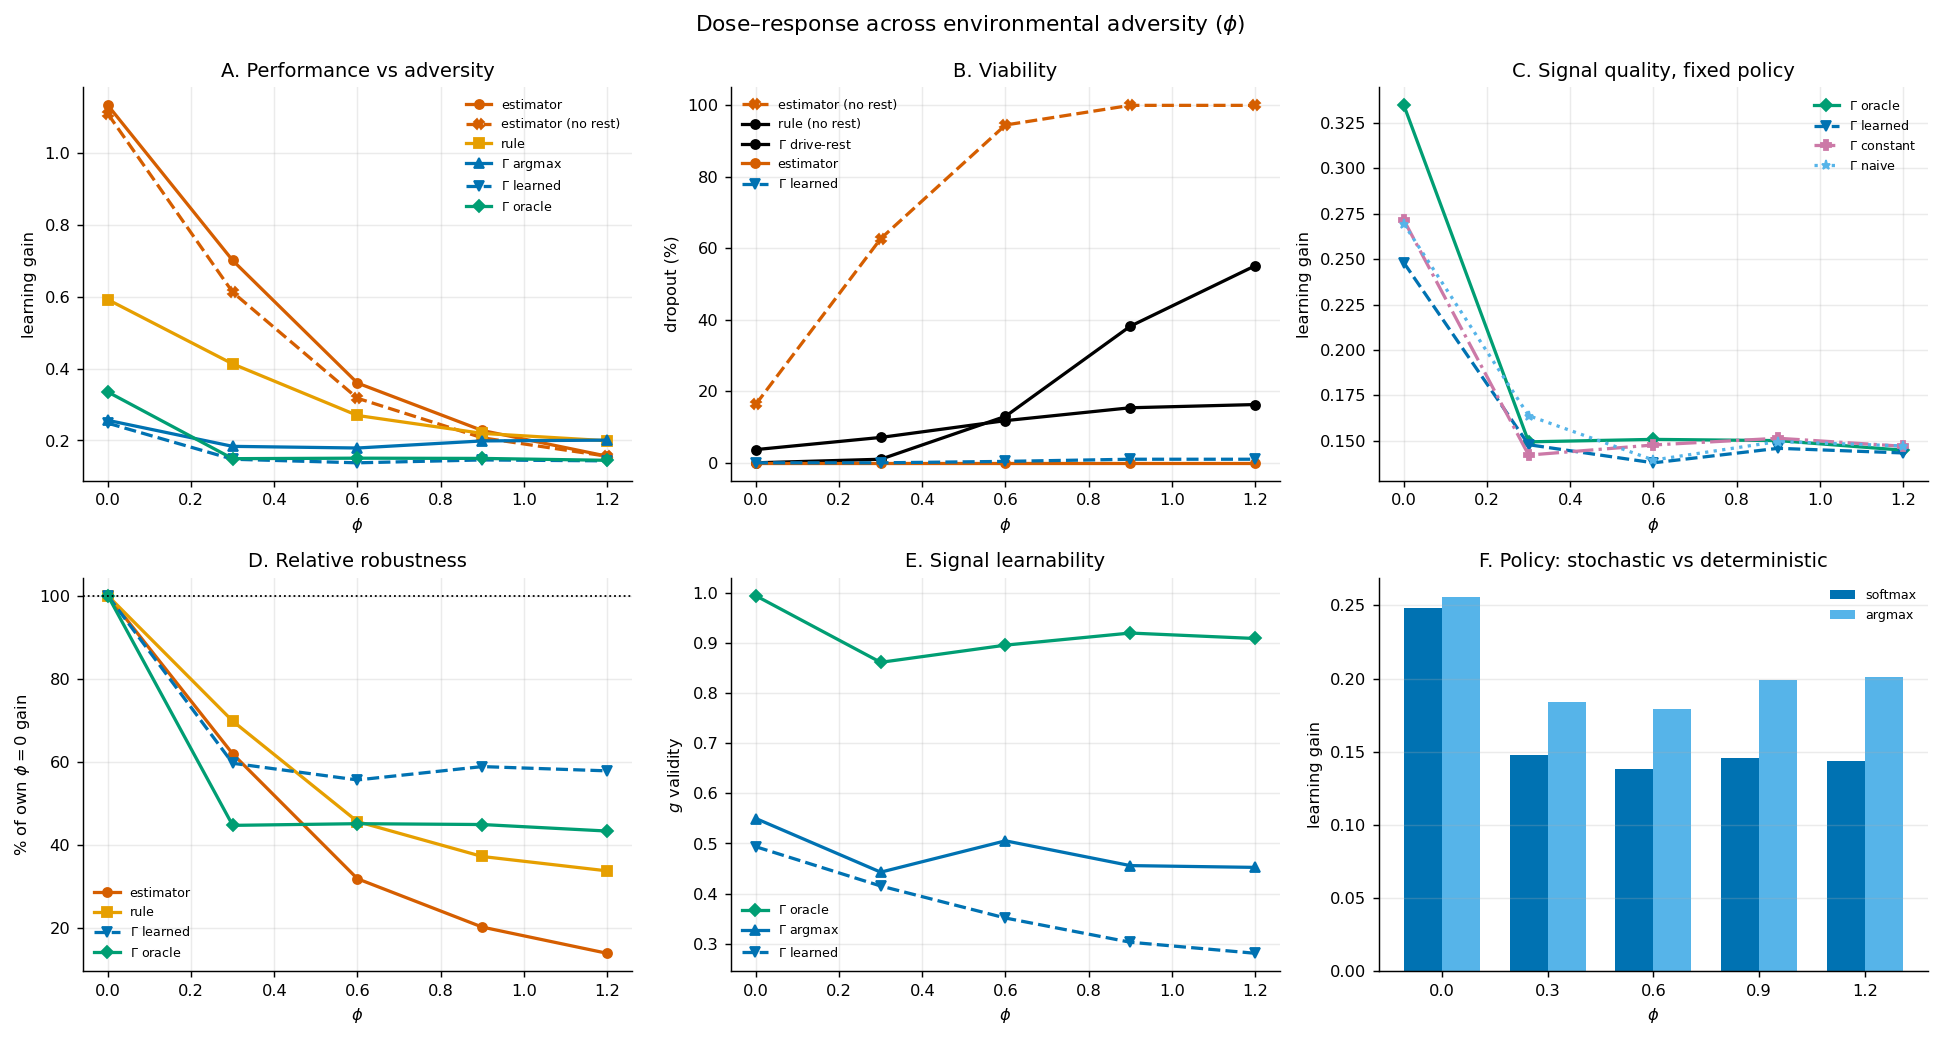
\includegraphics[width=\linewidth]{fig_v4.png}
  \caption{Six-panel summary, Okabe-Ito colourblind-safe palette with distinct markers and line styles so the panels remain legible in greyscale. \textbf{A}: performance across adversity. \textbf{B}: viability. \textbf{C}: signal quality under the fixed hand policy. \textbf{D}: robustness normalized to each arm's own $\phi{=}0$ value. \textbf{E}: signal learnability. \textbf{F}: stochastic versus deterministic policy.}
\end{figure}

\section{Compute resources and LLM usage}
\label{app:compute}
\label{app:compute}

All experiments run on a commodity laptop with no GPU; the main sweep of 60{,}000 episodes takes $31.4$ s single-threaded and a single decision costs $14$ $\mu$s (full specifications in Appendix~\ref{app:compute}).

We disclose LLM usage for transparency, although it is not a component of the core method: no language model participates in the agent, the environment, the baselines, or the analysis, all of which are explicit numerical simulations. LLMs served as engineering assistants in two capacities --- code assistance, via Devin as an IDE together with Kimi 3 and DeepSeek v4 Pro, and Claude Opus 5 and Claude Fable 5; and writing and editing assistance, via Claude Opus 5 and Claude Fable 5. All experimental design decisions, the committed predictions, the statistical procedures, and every interpretation are the authors' own, and all reported numbers were produced by executing the released notebook.


\section{Reproducibility}
\label{app:repro}
Ten seeds are derived from master seed \texttt{20260820} via SHA-256, each mapped to the next prime above $10007+(\text{digest}\bmod 900000)$; profiles come from a separate fixed seed. The released notebook reproduces every reported number and asserts the prediction hash before running. Dependencies are \texttt{scipy} and \texttt{matplotlib}.

\section{Preregistered prediction text (verbatim)}
\label{app:prereg}
The authoritative artifact is \texttt{predictions.txt} in the supplement, whose SHA-256 digest is \texttt{6e888c7e46e1dd306b6adc601a45cc08ff914a24d2f474a913a1ff2907bfc084}. It contains one prediction per line in sorted key order, joined with newlines. Below the same text is shown with display-only wrapping; continuation lines are indented and are \emph{not} part of the hashed string.
{\footnotesize
\begin{verbatim}
P1: bayesian_norest (estimacion sin gestion de viabilidad) colapsa al subir
    phi: dropout alto, gain al piso.
P2: Los brazos Gamma se degradan proporcionalmente menos que el bayesiano a
    lo largo del barrido de phi.
P3: Existe phi* dentro del rango valido de la puerta de calidad donde algun
    brazo Gamma supera al bayesiano en gain.
P4: gamma_learned_argmax supera a gamma_learned en todos los puntos validos
    del barrido.
P5: Si la calidad de g se transmite a la conducta, gamma_oracle se separa de
    gamma_no_learning en algun punto del barrido.
P6: g_validity de gamma_learned decrece monotonamente al subir phi.
P7: Bajo desplazamiento del PICO de la campana de aprendizaje (cambio de
    forma, no de escala), los brazos Gamma ganan terreno relativo frente al
    bayesiano, que queda mal especificado y no puede absorberlo re-estimando h.
\end{verbatim}
}

\section{Source code}
\label{app:code}
Self-contained: no external dataset, no pretrained model, only \texttt{scipy} and \texttt{matplotlib} beyond the standard library. \textbf{Naming note:} the code predates the paper's terminology --- \texttt{BayesianAgent} is the paper's \emph{estimator}, \texttt{BayesianNoObjAgent} the estimator without an objective model, \texttt{ReglaAgent} the \emph{rule}, \texttt{gamma\_no\_learning} the \emph{constant-$g$} arm; \texttt{nivel}, \texttt{ganancia} and \texttt{descansar} are level, gain and rest.
\footnotesize
\subsection{Seeds and determinism}
\begin{verbatim}
import hashlib, math, random
from collections import defaultdict

NIVELES=[1,2,3,4,5]
PRESUPUESTO=40
E_REF=3.0

def _is_prime(n):
    if n<2: return False
    if n in (2,3,5,7): return True
    if n%2==0 or n%3==0: return False
    i=5
    while i*i<=n:
        if n%i==0 or n%(i+2)==0: return False
        i+=6
    return True
def _next_prime(n):
    if n<=2: return 2
    c=n|1
    while not _is_prime(c): c+=2
    return c
def derive_seeds(master,n=10):
    s=[]
    for i in range(n):
        d=hashlib.sha256(f"{master}:run_{i}".encode()).hexdigest()
        s.append(_next_prime(10007+int(d,16)%900000))
    return s

def rasch_p(h,nivel): return 1.0/(1.0+math.exp(-1.5*(h-nivel)))
PEAK_MODEL=0.5   # peak assumed by any agent that models the curve (misspecifiable)
def bell_curve(gap,peak=PEAK_MODEL): return 0.08*math.exp(-((gap-peak)**2)/0.5)
\end{verbatim}
\subsection{Environment}
\begin{verbatim}
class StudyEnv:
    """v4: fatiga normalizada + histeresis + shift de regimen + examen en h_eff."""
    def __init__(self, h0, lr_mult=1.0, phi=0.0, lambda_olv=0.01,
                 hysteresis=False, e_crit=1.3, shift_mult=1.0, shift_at=20,
                 peak_gap=PEAK_MODEL, peak_new=None, peak_at=20):
        self.h=h0; self.h0=h0; self.lr_mult=lr_mult
        self.phi=phi; self.phi0=phi
        self.lambda_olv=lambda_olv
        self.hysteresis=hysteresis; self.e_crit=e_crit
        self.shift_mult=shift_mult; self.shift_at=shift_at
        self.peak_gap=peak_gap; self.peak_new=peak_new; self.peak_at=peak_at
        self.esfuerzo=0.0

    def tick(self,s):
        if self.shift_mult!=1.0 and s==self.shift_at:
            self.phi=self.phi0*self.shift_mult
        if self.peak_new is not None and s==self.peak_at:
            self.peak_gap=self.peak_new

    @property
    def esf_n(self): return self.esfuerzo/E_REF
    @property
    def h_eff(self): return max(0.5, self.h - self.phi*self.esf_n**1.5)
    @property
    def lr_eff(self):
        # la fatiga degrada la CAPACIDAD de aprender, no solo la dificultad aparente
        return self.lr_mult*max(0.15, 1.0 - 0.7*self.phi*self.esf_n**1.5)

    def expected_gain(self,nivel):
        gap=nivel-self.h_eff; p=rasch_p(self.h_eff,nivel)
        return bell_curve(gap,self.peak_gap)*(p*1.0+(1-p)*0.3)*self.lr_eff
    def in_zpd(self,nivel):
        g=[self.expected_gain(k) for k in NIVELES]; mx=max(g)
        return (self.expected_gain(nivel)>=0.5*mx) if mx>0 else False

    def exercise(self,nivel,rng):
        p=rasch_p(self.h_eff,nivel)
        correcto=rng.random()<p
        gap=max(0.0,nivel-self.h_eff)
        latencia=rng.lognormvariate(math.log(5)+0.6*gap,0.4)
        self.esfuerzo=0.95*self.esfuerzo+latencia/20.0
        gain=bell_curve(nivel-self.h_eff,self.peak_gap)*(1.0 if correcto else 0.3)*self.lr_eff
        self.h=min(6.0,self.h+gain)
        return {"correcto":correcto,"latencia":round(latencia,2),"gain":gain}

    def descansar(self):
        if self.hysteresis and self.esf_n>self.e_crit: self.esfuerzo*=0.93
        else: self.esfuerzo*=0.7
        self.h=max(0.5,self.h-self.lambda_olv)
\end{verbatim}
\subsection{Homeostatic agent}
The coupling uses the \emph{receiving} drive's pressure, matching Eq.~(1); the legacy sender-modulated branch is kept for reference only and used for no reported result.
\begin{verbatim}
class GCfg:
    def __init__(self,**kw):
        self.lam_p=kw.get("lam_p",0.15); self.lam_c=kw.get("lam_c",0.02)
        self.theta=kw.get("theta",0.7)
        self.alpha_p=kw.get("alpha_p",0.3); self.alpha_c=kw.get("alpha_c",0.3)
        self.w_cp=kw.get("w_cp",-0.05); self.w_pc=kw.get("w_pc",0.05)
        self.g_mode=kw.get("g_mode","learned")
        self.n_drives=kw.get("n_drives",2); self.coupling=kw.get("coupling",True)
        self.coupling_mode=kw.get("coupling_mode",
                "receiver")  # receiver (Eq.1 / design intent) | sender (legacy bug)
        self.eta=kw.get("eta",0.3); self.beta=kw.get("beta",0.2)
        self.g_init_p=kw.get("g_init_p",0.3); self.g_init_c=kw.get("g_init_c",0.5)
        self.g_naive=kw.get("g_naive",0.5)
        self.action_mode=kw.get("action_mode","softmax")   # softmax | argmax
        self.rest_mode=kw.get("rest_mode","gated")  # gated | drive | none
        self.coef=kw.get("coef",(4.0,-3.0,-3.0,1.5,4.0,-3.0))  # up_p,up_c,stay_k,stay_b,down_c,
                down_p          # gated | drive

class GammaAgent:
    def __init__(self,cfg,profile):
        self.cfg=cfg; self.p=profile
        self.d_prog=0.5; self.d_conf=0.5
        self.g_prog={k:cfg.g_init_p for k in NIVELES}
        self.g_conf={k:cfg.g_init_c for k in NIVELES}
        self.acc_ema={}; self.nivel=1; self.frust=0.0
        self.consec_high=0; self.abandono=False; self.dropout_session=None
    def _pressure(self,d): return min(1.0,abs(d-self.cfg.theta)/0.8)
    def basal(self):
        m=self.acc_ema.get(self.nivel,0.5)
        self.d_prog=min(2.0,self.d_prog+self.cfg.lam_p*m)
        if self.cfg.n_drives>=2:
            self.d_conf=min(2.0,self.d_conf+self.cfg.lam_c)
            if self.cfg.coupling:
                pc=self._pressure(self.d_conf); pp=self._pressure(self.d_prog)
                if self.cfg.coupling_mode=="receiver":
                    # Eq.(1): modulated by the RECEIVING drive's own pressure
                    m_to_prog, m_to_conf = pp, pc
                else:
                    m_to_prog, m_to_conf = pc, pp     # legacy: sender's pressure
                if self.d_conf>self.cfg.theta+0.05:
                    self.d_prog=max(0.0,self.d_prog+self.cfg.w_cp*m_to_prog)
                if self.d_prog>self.cfg.theta+0.05:
                    self.d_conf=max(0.0,self.d_conf+self.cfg.w_pc*m_to_conf)
    def select(self,rng,env):
        th=self.cfg.theta
        dp=self.d_prog-th
        dc=(self.d_conf-th) if self.cfg.n_drives>=2 else 0.0
        fn=self.frust/max(self.p["umbral"],0.1)
        strain=max(0.0,fn-0.7)/0.3
        if self.cfg.n_drives>=2:
            if self.cfg.rest_mode=="gated":
                l_rest=2*max(0.0,dc)*strain+4*strain
            elif self.cfg.rest_mode=="none":
                l_rest=-1e9          # rest unavailable: isolates drives from the frustration
                        gate
            else:
                l_rest=3.0*max(0.0,dc)+2.0*strain-1.2
            c=self.cfg.coef
            logits=[c[0]*dp+c[1]*dc, c[2]*(abs(dp)+abs(dc))+c[3], c[4]*dc+c[5]*dp, l_rest]
        else:
            logits=[4*dp,-3*abs(dp)+1.5,-4*dp,4*strain]
        acts=["subir","mantener","bajar","descansar"]
        if self.cfg.action_mode=="argmax":
            return acts[max(range(4),key=lambda i:logits[i])]
        mx=max(logits); exps=[math.exp(min(50,l-mx)) for l in logits]
        tot=sum(exps); r=rng.random()*tot; cum=0.0
        for i,e in enumerate(exps):
            cum+=e
            if r<cum: return acts[i]
        return "mantener"
    def study(self,env,outcome,nivel):
        c=outcome["correcto"]; eb=self.acc_ema.get(nivel,0.5)
        self.acc_ema[nivel]=(1-self.cfg.beta)*eb+self.cfg.beta*float(c)
        if self.cfg.g_mode=="learned":
            a=self.acc_ema[nivel]
            self.g_prog[nivel]=(1-self.cfg.eta)*self.g_prog[nivel]+self.cfg.eta*(4.0*a*(1.0-a))
            self.g_conf[nivel]=(1-self.cfg.eta)*self.g_conf[nivel]+self.cfg.eta*a
        elif self.cfg.g_mode=="oracle":
            self.g_prog[nivel]=min(1.0,env.expected_gain(nivel)/0.042)
            self.g_conf[nivel]=rasch_p(env.h_eff,nivel)
        if self.cfg.g_mode=="naive": gp=gc=self.cfg.g_naive
        else: gp=self.g_prog[nivel]; gc=self.g_conf[nivel]
        if c:
            self.d_prog=max(0.0,self.d_prog-self.cfg.alpha_p*gp)
            if self.cfg.n_drives>=2:
                self.d_conf=max(0.0,self.d_conf-self.cfg.alpha_c*gc)
            if outcome["latencia"]<15: self.frust=max(0.0,self.frust-0.35)
        else:
            if self.cfg.n_drives>=2: self.d_conf=min(2.0,self.d_conf+0.1)
            self.frust+=0.25
            if eb>=0.7: self.frust+=0.3
\end{verbatim}
\subsection{Baselines}
\begin{verbatim}
class ReglaAgent:
    def __init__(self,profile,rest=True):
        self.p=profile; self.rest=rest; self.nivel=1; self.frust=0.0
        self.consec_high=0; self.abandono=False; self.dropout_session=None
        self.streak_c=0; self.streak_e=0; self.acc_ema={}
    def select(self,rng,env):
        if self.rest and self.frust>0.6*self.p["umbral"]: return "descansar"
        if self.streak_e>=2: return "bajar"
        if self.streak_c>=3: return "subir"
        return "mantener"
    def study(self,env,outcome,nivel):
        if outcome["correcto"]: self.streak_c+=1; self.streak_e=0
        else: self.streak_e+=1; self.streak_c=0

class BayesianNoObjAgent:
    """State estimation WITHOUT an objective model: tracks h_hat from outcomes and
    simply matches the level to estimated ability. Isolates estimation from
    privileged knowledge of where the learning curve peaks."""
    def __init__(self,profile,rest=True):
        self.p=profile; self.rest=rest; self.nivel=1; self.h_hat=2.5
        self.frust=0.0; self.consec_high=0; self.abandono=False
        self.dropout_session=None; self.acc_ema={}
    def select(self,rng,env):
        if self.rest and self.frust>0.6*self.p["umbral"]: return "descansar"
        best=min(NIVELES,key=lambda k: abs(k-self.h_hat))
        if best>self.nivel: return "subir"
        if best<self.nivel: return "bajar"
        return "mantener"
    def study(self,env,outcome,nivel):
        p=rasch_p(self.h_hat,nivel)
        self.h_hat+=0.3*(float(outcome["correcto"])-p)
        self.h_hat=max(0.5,min(6.0,self.h_hat))

class BayesianAgent:
    def __init__(self,profile,rest=True):
        self.p=profile; self.rest=rest; self.nivel=1; self.h_hat=2.5
        self.frust=0.0; self.consec_high=0; self.abandono=False
        self.dropout_session=None; self.acc_ema={}
    def select(self,rng,env):
        if self.rest and self.frust>0.6*self.p["umbral"]: return "descansar"
        best,bg=self.nivel,-1
        for k in NIVELES:
            gap=k-self.h_hat; p=rasch_p(self.h_hat,k)
            g=bell_curve(gap)*(p+(1-p)*0.3)
            if g>bg: best,bg=k,g
        if best>self.nivel: return "subir"
        if best<self.nivel: return "bajar"
        return "mantener"
    def study(self,env,outcome,nivel):
        p=rasch_p(self.h_hat,nivel)
        self.h_hat+=0.3*(float(outcome["correcto"])-p)
        self.h_hat=max(0.5,min(6.0,self.h_hat))

class FixedAgent:
    def __init__(self,profile,mode):
        self.p=profile; self.mode=mode; self.nivel=1; self.frust=0.0
        self.consec_high=0; self.abandono=False; self.dropout_session=None
        self.acc_ema={}
    def select(self,rng,env):
        if self.mode=="always1": t=1
        elif self.mode=="always5": t=5
        elif self.mode=="random": t=rng.choice(NIVELES)
        else: t=max(NIVELES,key=lambda k:env.expected_gain(k))
        if t>self.nivel: return "subir"
        if t<self.nivel: return "bajar"
        return "mantener"
    def study(self,env,outcome,nivel): pass

def shared_frust_update(agent,outcome,eb):
    if outcome["correcto"]:
        if outcome["latencia"]<15: agent.frust=max(0.0,agent.frust-0.35)
    else:
        agent.frust+=0.25
        if eb>=0.7: agent.frust+=0.3
\end{verbatim}
\subsection{Profiles and episode runner}
\begin{verbatim}
def gen_profiles(n=100,seed=2026):
    rng=random.Random(seed)
    return [{"h0":round(rng.uniform(1.5,3.5),2),
             "lr_mult":round(rng.uniform(0.7,1.3),2),
             "umbral":round(rng.uniform(1.8,3.0),1)} for _ in range(n)]

def run_episode(agent,profile,seed,is_gamma,env_kw,log=False):
    env=StudyEnv(profile["h0"],lr_mult=profile["lr_mult"],**env_kw)
    rng=random.Random(seed); traj=[]; zpd=0; nst=0; ndesc=0; s=0
    for s in range(PRESUPUESTO):
        if agent.abandono: break
        env.tick(s)
        if is_gamma: agent.basal()
        a=agent.select(rng,env)
        if a=="subir": agent.nivel=min(5,agent.nivel+1)
        elif a=="bajar": agent.nivel=max(1,agent.nivel-1)
        out=None; inz=False
        if a=="descansar":
            env.descansar(); agent.frust*=0.5; ndesc+=1
        else:
            inz=env.in_zpd(agent.nivel)
            out=env.exercise(agent.nivel,rng); nst+=1
            if inz: zpd+=1
            if is_gamma: agent.study(env,out,agent.nivel)
            else:
                eb=agent.acc_ema.get(agent.nivel,0.5)
                agent.acc_ema[agent.nivel]=0.8*eb+0.2*float(out["correcto"])
                shared_frust_update(agent,out,eb)
                agent.study(env,out,agent.nivel)
        if agent.frust>=0.95*profile["umbral"]: agent.consec_high+=1
        else: agent.consec_high=0
        if agent.consec_high>=3 and not agent.abandono:
            agent.abandono=True; agent.dropout_session=s
        if log:
            traj.append({"s":s,"nivel":agent.nivel,"action":a,
                "correcto":out["correcto"] if out else None,
                "d_prog":round(getattr(agent,"d_prog",0),3),
                "d_conf":round(getattr(agent,"d_conf",0),3),
                "frust":round(agent.frust,2),"h":round(env.h,3),
                "h_eff":round(env.h_eff,3),"esf_n":round(env.esf_n,3),"in_zpd":inz})
    m={"ganancia":round(env.h-profile["h0"],3),
       "h_final":round(env.h,3),
       "exam":round(rasch_p(env.h,3),3),
       "exam_taken":round(0.0 if agent.abandono else rasch_p(env.h_eff,3),3),
       "exam_eff":round(rasch_p(env.h_eff,3),3),
       "esf_n_final":round(env.esf_n,3),
       "tiz":round(zpd/max(1,nst),3),
       "tib_full":round(zpd/PRESUPUESTO,3),
       "dropout":agent.abandono,"dropout_session":agent.dropout_session,
       "n_descansar":ndesc,"n_study":nst,"nivel_final":agent.nivel,
       "sessions_used":s+1}
    if is_gamma and agent.cfg.g_mode in ("learned","oracle","fixed","naive"):
        gains=[env.expected_gain(k) for k in NIVELES]
        gps=[agent.g_prog[k] for k in NIVELES]
        mg=sum(gains)/5; mp=sum(gps)/5
        cov=sum((gains[i]-mg)*(gps[i]-mp) for i in range(5))
        vg=math.sqrt(sum((g-mg)**2 for g in gains)); vp=math.sqrt(sum((g-mp)**2 for g in gps))
        m["g_validity"]=round(cov/(vg*vp),3) if vg>0 and vp>0 else None
        m["g_prog_final"]={str(k):round(agent.g_prog[k],3) for k in NIVELES}
        m["true_gain_final"]={str(k):round(env.expected_gain(k),4) for k in NIVELES}
    return m,traj

CFG_BASE=dict(lam_p=0.15,alpha_p=0.3,alpha_c=0.3,theta=0.7)
\end{verbatim}
\normalsize

\section{Analysis code: paired inference and equivalence}
\label{app:paired}
The design is within-subject --- the same 100 profiles face every arm --- so contrasts are paired and equivalence is tested explicitly rather than inferred from non-significance.
\begin{verbatim}
from scipy.stats import ttest_rel, t as tdist

def per_profile(arm, phi):                  # one unit per profile
    return [mean(run(arm, profile, seed, phi) for seed in SEEDS)
            for profile in PROFILES]

def paired_contrast(a, b, phi):
    xa, xb = per_profile(a, phi), per_profile(b, phi)
    d  = [u - v for u, v in zip(xa, xb)]
    n  = len(d); m = mean(d); se = stdev(d) / sqrt(n)
    h  = se * tdist.ppf(0.975, n - 1)       # 95% CI half-width
    t, p = ttest_rel(xa, xb)                # NOT ttest_ind: paired design
    return m, (m - h, m + h), p, m / stdev(d)

def tost(d, delta):                         # two one-sided tests
    n = len(d); m = mean(d); se = stdev(d) / sqrt(n)
    return max(1 - tdist.cdf((m + delta) / se, n - 1),
                   tdist.cdf((m - delta) / se, n - 1))

# P3 is an existence claim: max-statistic sign-flip permutation
T_obs = max(paired_t(arm, phi) for arm in GAMMA_ARMS for phi in PHIS_VALID)
null  = [max(paired_t(arm, phi, flip=s) for arm in GAMMA_ARMS
             for phi in PHIS_VALID) for s in random_sign_flips(2000)]
p_P3  = (sum(t >= T_obs for t in null) + 1) / 2001
\end{verbatim}

\newpage
\input{checklist.tex}

\end{document}
